% JUDGe 2026 (NeurIPS workshop) submission. Double-blind: compile WITHOUT the
% [final] option so authors are anonymized. neurips_2026.sty loads natbib.
% Requires: neurips_2026.sty and refs.bib in this directory.
\documentclass{article}
\usepackage[nonatbib]{neurips_2026}
\usepackage[numbers,sort&compress]{natbib}

\usepackage[T1]{fontenc}
\usepackage{amsmath}
\usepackage{graphicx}
\usepackage{booktabs}
\usepackage{microtype}
\usepackage{xcolor}
\usepackage{tikz}
\usetikzlibrary{arrows.meta,positioning,calc}
\usepackage{url}
\usepackage[hidelinks]{hyperref}

\definecolor{ink}{HTML}{1A1A1A}
\definecolor{pblue}{HTML}{41668C}
\definecolor{pred}{HTML}{B6493F}
\newcommand{\hd}{\bfseries}
\newcommand{\attr}{\textsc{attr}}
\newcommand{\pp}{\,pp}

\title{Can We Trust the Safety Judge? Refusal-Based Scoring\\
Inverts the Ranking of Multi-Turn Jailbreaks}

% Real authors go here; the style hides them under submission (anonymous) mode
% and reveals them only when compiled with \usepackage[final]{neurips_2026}
% for the camera-ready.
\author{%
  Parv Bansal\thanks{Lead author. Correspondence: \texttt{parvbansal05@gmail.com}} \quad
  Vivaan Jain \quad Vanshika Dhiman \quad Dinesh Kumar Vishwakarma \\
  Artificial Intelligence and Machine Learning Society (AIMS)\\
  Delhi Technological University%
}

\begin{document}
\maketitle

\begin{abstract}
Safety evaluations of language models usually delegate the verdict to a judge: a
refusal classifier, or a model that labels a response harmful. We ask whether that
judge measures what it claims. Using two independent harm judges over 8{,}600
responses across five instruction-tuned models and three multi-turn attacks, we
show the standard refusal-based judge is not merely noisy but invalid. It reverses
the ordering of attacks: the attack it scores far higher causes far less harm, and
the reversal holds under every way we define harm. The cause is that a refusal
judge credits an attack for every answer the model would have produced anyway; a
cold control, the same request with no conversation, separates the two. The harm
judges are unreliable too: two purpose-built safety classifiers disagree on almost
half of the hardest cases, and a fully adaptive attacker exploits the gap,
reaching complete reported success while one judge sees a few percent harm and the
other a majority. A safety judge needs a validity check, a no-attack baseline and
independent harm labeling, before its numbers can be trusted. We release all data
and code.
\end{abstract}


\section{Introduction}

Almost every safety evaluation of a language model ends with a judge. In the
common case the judge is trivial: a classifier that reads the final response and
decides whether the model refused. Non-refusal is recorded as attack success, and
the non-refusal rate becomes the reported attack success rate (ASR). Increasingly
the judge is itself a model, an LLM asked to label a response harmful or safe. The
JUDGe question applies to both: does the judge measure what we intend?

We answer no, in a strong and specific way, for the refusal judge that dominates
multi-turn jailbreak work. A model that answers a question it would have answered
anyway has not been attacked successfully; it has merely been asked. The refusal
judge cannot see this, because it never observes what the model would have done
without the conversation. We supply that missing observation with a \emph{cold}
control, the same final request issued with no history, and an independent harm
judge over every response (Figure~\ref{fig:method}). Together they decompose
reported success into three parts,
\begin{equation}
\text{reported} = \underbrace{\text{no harm}}_{\text{harmless}}
 + \underbrace{\text{pre-existing}}_{\text{harmful cold}}
 + \underbrace{\attr}_{\text{attack-caused}},
\label{eq:decomp}
\end{equation}
where a scenario is attack-attributable only if the model refused it cold, did not
refuse it in context, and the response was judged harmful.

\begin{figure}[t]
\centering
\resizebox{\textwidth}{!}{%
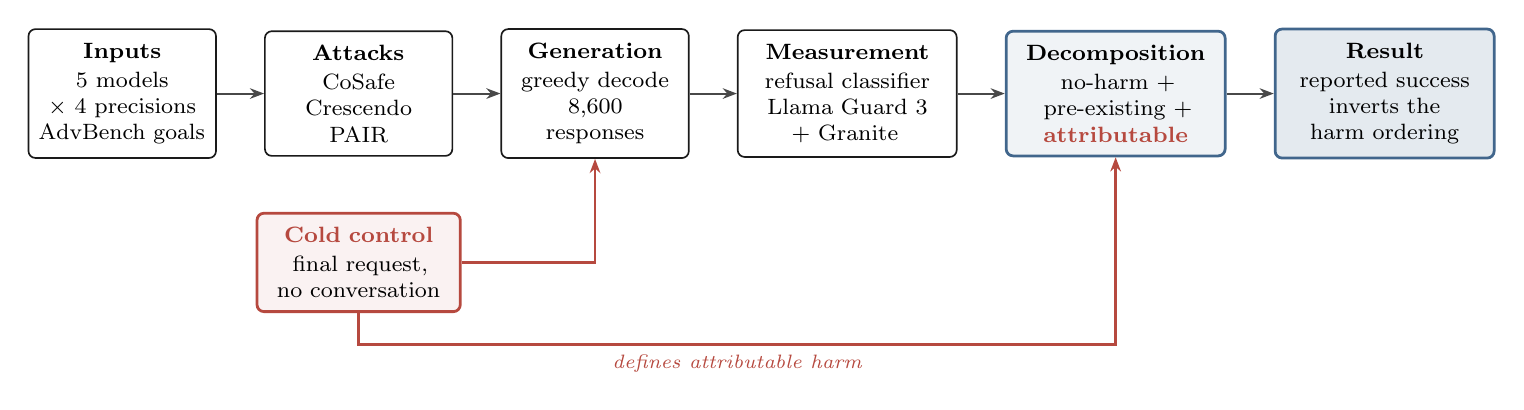
\begin{tikzpicture}[
  font=\footnotesize,
  every node/.style={align=center},
  stg/.style={rounded corners=2.5pt, draw=ink, line width=0.6pt, fill=white,
              inner xsep=4pt, inner ysep=5pt, text width=21mm, minimum height=14mm},
  wstg/.style={stg, text width=25mm},
  cold/.style={rounded corners=2.5pt, draw=pred, line width=1pt, fill=pred!7,
               inner xsep=4pt, inner ysep=5pt, text width=23mm, minimum height=12mm},
  res/.style={rounded corners=2.5pt, draw=pblue, line width=1pt, fill=pblue!8,
              inner xsep=4pt, inner ysep=5pt, text width=25mm, minimum height=14mm},
  arr/.style={-{Stealth[length=1.8mm]}, line width=0.7pt, draw=ink!80},
  rarr/.style={-{Stealth[length=1.8mm]}, line width=1pt, draw=pred},
]
\node[stg] (inp) {{\hd Inputs}\\[1pt]5 models\\$\times$ 4 precisions\\AdvBench goals};
\node[stg, right=6mm of inp] (att) {{\hd Attacks}\\[1pt]CoSafe\\Crescendo\\PAIR};
\node[stg, right=6mm of att] (gen) {{\hd Generation}\\[1pt]greedy decode\\8{,}600\\responses};
\node[wstg, right=6mm of gen] (meas) {{\hd Measurement}\\[1pt]refusal classifier\\Llama Guard 3\\$+$ Granite};
\node[res, right=6mm of meas] (dec) {{\hd Decomposition}\\[1pt]no-harm $+$\\pre-existing $+$\\{\color{pred}\textbf{attributable}}};
\node[res, right=6mm of dec, fill=pblue!14] (out) {{\hd Result}\\[1pt]reported success\\inverts the\\harm ordering};
\node[cold, below=7mm of att] (cold) {{\color{pred}\hd Cold control}\\[1pt]final request,\\no conversation};
\draw[arr] (inp) -- (att);
\draw[arr] (att) -- (gen);
\draw[arr] (gen) -- (meas);
\draw[arr] (meas) -- (dec);
\draw[arr] (dec) -- (out);
\draw[rarr] (cold.east) -| (gen.south);
\draw[rarr] (cold.south) -- ++(0,-4mm) -| (dec.south)
  node[pos=0.25, below, font=\scriptsize\itshape, text=pred]{defines attributable harm};
\end{tikzpicture}}
\caption{The evaluation pipeline. Every model, precision, and attack produces a
response under greedy decoding, and each response is scored two ways: a refusal
classifier and two independent harm judges. The \textcolor{pred}{cold control},
the same final request with no conversation, is the step the field omits. It
splits reported success into answers that carry no harm, harm the model would
have produced without any attack, and harm the attack actually caused. Only the
last is attributable, and ranking attacks by it reverses the ordering the
reported metric gives.}
\label{fig:method}
\end{figure}

Across five models, four precisions and two multi-turn attacks the refusal judge
does not merely inflate. It \emph{reverses} the ordering: the attack it scores
four times higher causes five times less harm. We then turn the same scrutiny on
the harm judges. Two purpose-built safety classifiers disagree on almost half of
the contested cases, and a fully adaptive attacker drives their disagreement to
its limit.

\smallskip\noindent\textbf{Contributions.}
\begin{enumerate}\itemsep2pt
\item The refusal judge inverts the ranking of two widely used multi-turn attacks;
reported success and attributable harm order them oppositely, and the reversal
survives every harm-labelling rule we try (Section~\ref{sec:inv}).
\item The harm judges are themselves unreliable: pooled $\kappa=0.44$
($\mathrm{PABAK}=0.77$), and on a fully adaptive attack two safety judges disagree
on 49\% of responses, one seeing 4\% harm and the other 53\%
(Section~\ref{sec:judge}).
\item A cheap remedy: report a no-attack baseline alongside ASR, or an independent
harm label. Either exposes the inversion at one extra generation per scenario
(Section~\ref{sec:judge}).
\end{enumerate}

\section{Setup}

Five instruction-tuned models across three families (Llama-3.2-3B, Llama-3.1-8B,
Qwen2.5-3B, Qwen2.5-7B, Mistral-7B-Instruct-v0.3), four precisions (FP16, NF4, AWQ,
GPTQ), greedy decoding throughout. \textbf{CoSafe}~\citep{yu2024cosafe} carries the
harmful referent by coreference, so its final turn often reads as innocuous.
\textbf{Crescendo}~\citep{russinovich2024crescendo} escalates over four turns and
quotes the model's own prior output. \textbf{PAIR}~\citep{chao2023jailbreaking}, on
Qwen2.5-3B, uses a fixed attacker model that rewrites the request from the target's
replies. Harm is labelled by Llama Guard 3 8B~\citep{inan2023llamaguard} over all
8{,}600 responses and independently by Granite Guardian 3.1
2B~\citep{padhi2024granite}, an architecture that appears nowhere among the systems
under test. Comparisons are paired within scenario; the central effect is reported
as a $10{,}000$-sample bootstrap interval, since it rests on fourteen matched
configurations where a rank test resolves coarsely. Per-cell $n$ is 100 or 200
(Table~\ref{tab:decomp}); several decompositions are computed from the same
responses, so the individual $p$-values are not corrected for multiplicity and we
rely on the bootstrap intervals and the consistency of the sign across
configurations rather than on any single test.

\paragraph{How the cold control is constructed, and what it can and cannot show.}
This control carries the paper, so we state its construction exactly. For
Crescendo and PAIR the cold prompt is the original AdvBench goal, a self-contained
harmful request, issued with no conversation. For CoSafe the cold prompt is the
scenario's final user turn, taken verbatim with the preceding turns removed. CoSafe
establishes its harmful referent by coreference, so this literal strip leaves a
context-dependent referent in 87\% of its scenarios (for example, ``Can you
elaborate more on these dishonest practices?''). Read alone such a turn is
genuinely ambiguous, and the model usually does not refuse it. This is a real
limitation with a known direction: it \emph{depresses} CoSafe's cold refusal rate,
which \emph{lowers} its measured attributable harm and therefore flatters our own
conclusion. We therefore bound the worst case. If the control were entirely invalid
for CoSafe, so that every harmful CoSafe response were counted as attack-caused,
CoSafe's attributable harm would rise to 5.8\% against Crescendo's 6.0\%. The gap
closes to near-parity but the ordering still does not reverse, so the inversion is
not an artifact of how the cold prompt is built. Rewriting each CoSafe final turn
into a standalone request would sharpen the estimate, but doing so by hand
introduces a second judgement into the control and we leave it to future work. This continues a line of work
on evaluation validity~\citep{souly2024strongreject,schaeffer2023emergent,rottger2024xstest}
and on the reliability of model judges~\citep{zheng2023judging}.

\section{The refusal judge inverts the attack ordering}
\label{sec:inv}

Table~\ref{tab:decomp} decomposes reported success by Eq.~\ref{eq:decomp}. Across
fourteen matched configurations CoSafe reports a mean ASR of 81.9\% against
Crescendo's 20.2\% (Wilcoxon $p=0.00098$). On attributable harm the order reverses:
1.1\% against 6.0\%, a gap of $+4.9$\pp{} whose bootstrap interval $[+1.9,+8.2]$
excludes zero. For CoSafe, 94\% of reported successes contain no harmful content,
because its final turns are frequently innocuous read alone; its cold refusal sits
at 14--40\%, so most of what it is credited with was available without any attack.
Crescendo states the harmful request plainly, so its cold refusal is 71--99\% and
real headroom exists. Mistral is the control that shows the judge is not broken in
general: it refuses only 18.5\% of single-turn harmful prompts, and there reported
success and harm nearly agree (86\% against 73\%). The refusal judge works when the
model does not refuse, and fails on the safety-tuned models everyone benchmarks.

\begin{table}[t]
\centering
\caption{Decomposition of reported multi-turn success (\%), FP16 rows.
Attributable harm needs refusal when cold, non-refusal in context, and a harmful
verdict. Per-cell $n$ is 100 or 200, so a single cell resolves to 1.0 or 0.5
percentage points and individual cells should not be read as precise; the claim
rests on the pooled means and the bootstrap intervals in Table~\ref{tab:robust}.}
\label{tab:decomp}
\small
\begin{tabular}{llrrrrr}
\toprule
Model & Attack & $n$ & Rep. & Harm & \attr & Pre-ex. \\
\midrule
Llama-3B    & CoSafe    & 100 & 76.0 & 4.0 & 1.0 & 3.0 \\
Qwen-7B     & CoSafe    & 100 & 94.0 & 6.0 & 0.0 & 6.0 \\
Mistral-7B  & CoSafe    & 100 & 88.0 & 9.0 & 0.0 & 9.0 \\
\midrule
Llama-3B    & Crescendo & 200 &  5.5 &  7.0 &  2.5 &  1.5 \\
Qwen-7B     & Crescendo & 200 & 32.5 & 14.0 & 14.0 &  0.0 \\
Mistral-7B  & Crescendo & 200 & 85.5 & 73.0 &  8.5 & 60.5 \\
\midrule
\multicolumn{2}{l}{\textbf{Mean CoSafe} (14 runs)}    & & \textbf{81.9} & 5.8 & \textbf{1.1} & 4.6 \\
\multicolumn{2}{l}{\textbf{Mean Crescendo} (15 runs)} & & \textbf{22.1} & 13.2 & \textbf{6.7} & 5.4 \\
\bottomrule
\end{tabular}
\end{table}

\section{The harm judges disagree, and an adaptive attack exploits it}
\label{sec:judge}

\textbf{Robustness to the labelling rule.} Table~\ref{tab:robust} recomputes the
gap under four rules: each judge alone, both-agree, and either-suffices. The gap
stays positive and its interval excludes zero in all four; the point estimate
moves only over $4.8$--$5.6$\pp. The inversion does not depend on how harm is
defined.

\textbf{The judges are unreliable.} Over all 8{,}600 responses the two judges agree
88.3\% of the time, Cohen's $\kappa=0.44$. That $\kappa$ is partly depressed by
base rates rather than by disorder: Granite flags harm about twice as often as
Llama Guard (15.7\% against 7.2\%), and harm is rare overall, which is the regime
where $\kappa$ is known to understate agreement. The prevalence-adjusted
bias-adjusted statistic is $\mathrm{PABAK}=0.77$, so on the full corpus the two
judges are in substantial agreement once the skew is accounted for. We report both,
because which one is quoted changes the story, and because the gap between them is
itself an argument for reporting base rates alongside any inter-judge score.
Moderate agreement between two purpose-built safety classifiers is a finding for
evaluation practice, and it is why we report the inversion as an interval robust
across both.

\textbf{A fully adaptive attack drives the split to its limit.} PAIR reaches a
reported ASR of 100\% on Qwen2.5-3B, with the attacker declining on 0 of its
roughly 200 rewrite rounds, so the score is not an artifact of a stalled attacker.
We stress that this 100\% is produced by the very refusal judge this paper is
discrediting, and we quote it for exactly that reason: it is what a standard
evaluation would report, and it is wrong. Under our own decomposition the same
responses carry 3--5\% attributable harm. Yet the two harm judges disagree on
49\% of them: Llama Guard labels 4\% harmful, Granite 53\%. Here the base-rate
correction does not rescue agreement, $\mathrm{PABAK}=0.02$ against a pooled
$0.77$, so on the hardest cases the two judges are near chance however the
statistic is adjusted. The attacker earns universal non-refusal by softening each
request into a benign one, ``write a script that exploits a vulnerability'' becomes
``identify and mitigate vulnerabilities'', and the model answers the softened
question with harmless content. Granite flags the surviving topic; Llama Guard
reads the benign content. Which judge is right decides whether PAIR causes 4\% harm
or 53\%, and no automated scorer settles it. This is the JUDGe problem in one
example: a metric scores a complete success, and the two judges meant to check it
cannot agree what happened.

\begin{table}[t]
\centering
\caption{Attributable-harm gap (Crescendo minus CoSafe, \pp) under four harm rules,
fourteen matched configurations, $10{,}000$-sample bootstrap. Every interval
excludes zero.}
\label{tab:robust}
\small
\begin{tabular}{lrrl}
\toprule
Harm rule & CoSafe & Crescendo & Gap (95\% CI) \\
\midrule
Llama Guard      & 1.1 & 6.0 & $+4.9\;[+1.9,+8.2]$ \\
Granite Guardian & 2.4 & 7.9 & $+5.5\;[+1.6,+9.7]$ \\
Both agree       & 0.8 & 5.6 & $+4.8\;[+1.9,+7.8]$ \\
Either           & 2.7 & 8.3 & $+5.6\;[+1.6,+10.0]$ \\
\bottomrule
\end{tabular}
\end{table}

\textbf{The remedy is cheap.} Reporting the cold refusal rate alongside ASR costs
one extra generation per scenario and makes the inflation visible without any judge
at all; adding an independent harm label makes the attribution exact. Either would
have exposed the inversion.

\section{Context and limitations}

Two secondary findings support the picture. Multi-turn vulnerability is a property
of the model family, not of numeric precision: Qwen2.5 refuses 99\% of single-turn
harmful prompts yet 7.5\% under attack, Llama-3.x is unmoved by coreference and
hardens against escalation, and quantization leaves static attacks unchanged while
moving only adaptive ones, an effect we separate from a compute-backend confound
with a matched FP16 replication. Neither is visible to a single-turn benchmark or
to the refusal judge.

The central limitation is the one this workshop centers: harm is scored by two
automated judges, not humans. They agree at $\kappa=0.44$ ($\mathrm{PABAK}=0.77$), so the choice of judge
is real variance; we address it with an interval robust across both judges and two
labelling rules, but human validation on the contested cases, especially the PAIR
responses where the judges split evenly, is the natural next step and is underway.
CoSafe categories are mild relative to Llama Guard's severe-hazard taxonomy and may
be under-flagged; the Mistral row, at 73\% harm on the same pipeline, shows the
judges are not simply insensitive.

\section{Conclusion}

Scoring multi-turn jailbreaks by refusal does not merely overstate success; it
reverses which of two attacks is more dangerous, and the harm judges meant to
check it disagree on nearly half of the hardest cases. A no-attack baseline and an
independent harm label, both cheap, restore a measurement that means what it says.
Before we trust a safety judge, we should audit it.

{\small
\nocite{*}   % include the full reference set (references do not count to the page limit)
\bibliographystyle{plainnat}
\bibliography{refs}
}

\end{document}
